\subsubsection{UC\theuccount-GP - Inserimento utente}
		\begin{figure}[H]
			\centering
				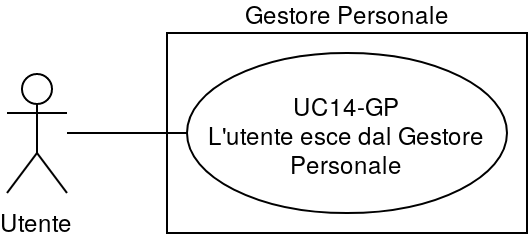
\includegraphics[width=\columnwidth]{img/casi_d'uso/UC14.png}\\
			\caption{UC\theuccount-GP - Inserimento utente}
		\end{figure}
	\begin{itemize}
		\item \textbf{Codice}: UC\theuccount-GP.
		\item \textbf{Titolo}: Inserimento utente.
		\item \textbf{Attori primari}: utente.
		\item \textbf{Descrizione}: l'utente, acceduto al sistema, aggiunge un nuovo utente nel sistema.
		Non è possibile che un utente non acceduto si iscriva da solo per la prima volta.
		In un primo momento è presente solo un utente predefinito che può aggiungere gli altri utenti.
		\item \textbf{Precondizione}: un nuovo utente deve essere aggiunto nel sistema.
		\item \textbf{Postcondizione}: un utente viene aggiunto al sistema.
		\item \textbf{Scenario principale}:
		\begin{enumerate}
			\item L'utente aggiunge un nuovo utente
		\end{enumerate}
	\end{itemize}
	%TODO:  aggiuora io, povero stronzo, che sono statonto.. come faccio a sapere qual è il mio identificativo?!
	\stepcounter{subuccount}
	\subsubsection{UC\theuccount.\thesubuccount-GP - Aggiunta nuovo utente}
		\begin{figure}[H]
			\centering
			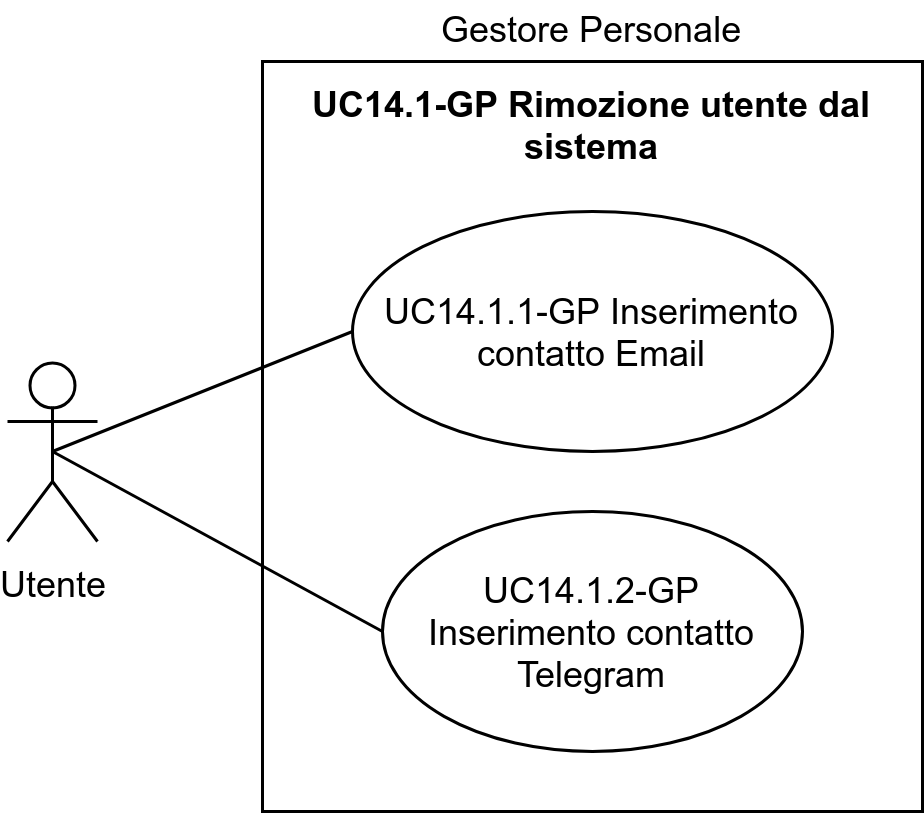
\includegraphics[width=\columnwidth]{img/casi_d'uso/UC14_1.png}\\
			\caption{UC\theuccount.\thesubuccount-GP - Aggiunta nuovo utente}
		\end{figure}
		\begin{itemize}
			\item \textbf{Codice}: C\theuccount.\thesubuccount-GP.
			\item \textbf{Titolo}: Aggiunta nuovo utente.
			\item \textbf{Attori primari}: utente.
			\item \textbf{Descrizione}: un nuovo utente viene inserito nel sistema.
			\item \textbf{Precondizione}: un nuovo utente deve essere aggiunto nel sistema.
			\item \textbf{Postcondizione}: un utente viene aggiunto al sistema.
			\item \textbf{Scenario principale}:
			\begin{enumerate}
				\item L'utente inserisce i dati del nuovo utente da aggiungere
				\item L'utente conferma l'invio dei dati
				\item L'aggiunta viene effettuata
			\end{enumerate}
			\item \textbf{Estensioni}:
			\begin{enumerate}
				\item Errore utente già presente nel sistema [UC\theuccount.2-GP]
			\end{enumerate}
		\end{itemize}

		\stepcounter{subsubuccount}
		\subsubsection{UC\theuccount.\thesubuccount.\thesubsubuccount-GP - Inserimento nome utente}

			\begin{itemize}
				\item \textbf{Codice}: UC\theuccount.\thesubuccount.\thesubsubuccount-GP.
				\item \textbf{Titolo}: inserimento nome utente.
				\item \textbf{Attori primari}: utente.
				%non registrato.
				\item \textbf{Descrizione}: l'utente inserisce il nominativo dell'utente da aggiungere.
				\item \textbf{Precondizione}: un nuovo utente deve essere aggiunto nel sistema.
				\item \textbf{Postcondizione}: il nome del nuovo utente è stato aggiunto nel sistema.
				\item \textbf{Scenario principale}:
				\begin{enumerate}
					\item L'utente aggiunge il nominativo del nuovo utente
				\end{enumerate}
			\end{itemize}

		\stepcounter{subsubuccount}
		\subsubsection{UC\theuccount.\thesubuccount.\thesubsubuccount-GP - Inserimento cognome utente}

			\begin{itemize}
				\item \textbf{Codice}: UC\theuccount.\thesubuccount.\thesubsubuccount-GP.
				\item \textbf{Titolo}: inserimento cognome utente.
				\item \textbf{Attori primari}: utente.
				% non registrato.
				\item \textbf{Descrizione}: l'utente inserisce il cognome dell'utente da aggiungere.
				\item \textbf{Precondizione}: un nuovo utente deve essere aggiunto nel sistema.
				\item \textbf{Postcondizione}: il cognome del nuovo utente è stato aggiunto nel sistema.
				\item \textbf{Scenario principale}:
				\begin{enumerate}
					\item L'utente aggiunge il cognome del nuovo utente
				\end{enumerate}
			\end{itemize}

		\stepcounter{subsubuccount}
		\subsubsection{UC\theuccount.\thesubuccount.\thesubsubuccount-GP - Inserimento contatto Email}

			\begin{itemize}
				\item \textbf{Codice}: UC\theuccount.\thesubuccount.\thesubsubuccount-GP.
				\item \textbf{Titolo}: inserimento contatto Email.
				\item \textbf{Attori primari}: utente.
				% non registrato.
				\item \textbf{Descrizione}: l'utente inserisce il contatto Email dell'utente da aggiungere. L'inserimento di questo campo è opzionale, ma è obbligatorio che l'utente da aggiungere possieda un contatto Email o un ID Telegram.
				\item \textbf{Precondizione}: un nuovo utente deve essere aggiunto nel sistema.
				\item \textbf{Postcondizione}: il contatto Email è stato aggiunto.
				\item \textbf{Scenario principale}:
				\begin{enumerate}
					\item L'utente aggiunge il contatto Email del nuovo utente
				\end{enumerate}
		\end{itemize}

		\stepcounter{subsubuccount}
		\subsubsection{UC\theuccount.\thesubuccount.\thesubsubuccount-GP - Inserimento contatto Telegram}

			\begin{itemize}
				\item \textbf{Codice}: UC\theuccount.\thesubuccount.\thesubsubuccount-GP.
				\item \textbf{Titolo}: inserimento contatto Telegram.
				\item \textbf{Attori primari}: utente.
				% non registrato.
				\item \textbf{Descrizione}: l'utente inserisce il contatto Telegram dell'utente da aggiungere. L'inserimento di questo campo è opzionale, ma è obbligatorio che l'utente da aggiungere possieda un contatto Email o un ID Telegram.
				\item \textbf{Precondizione}: un nuovo utente deve essere aggiunto nel sistema.
				\item \textbf{Postcondizione}: il contatto Telegram è stato aggiunto.
				\item \textbf{Scenario principale}:
				\begin{enumerate}
					\item L'utente aggiunge il contatto Telegram del nuovo utente
				\end{enumerate}
			\end{itemize}

	\stepcounter{subuccount}
	\subsubsection{UC\theuccount.\thesubuccount-GP - Errore utente già presente nel sistema}

		\begin{itemize}
			\item \textbf{Codice}: UC\theuccount.\thesubuccount-GP.
			\item \textbf{Titolo}: errore utente già presente nel sistema.
			\item \textbf{Attori primari}: utente.
			\item \textbf{Descrizione}: l’utente viene avvisato che i contatti Telegram o Email immessi non sono univoci.
			\item \textbf{Precondizione}: un nuovo utente deve essere aggiunto nel sistema.
			\item \textbf{Postcondizione}: il sistema comunica all’utilizzatore l’errore e l'utente non viene inserito.
			\item \textbf{Scenario principale}:
			\begin{enumerate}
				\item L'utente visualizza il messaggio d'errore
			\end{enumerate}
			\end{itemize}